\documentclass[1p]{elsarticle_modified}
%\bibliographystyle{elsarticle-num}

%\usepackage[colorlinks]{hyperref}
%\usepackage{abbrmath_seonhwa} %\Abb, \Ascr, \Acal ,\Abf, \Afrak
\usepackage{amsfonts}
\usepackage{amssymb}
\usepackage{amsmath}
\usepackage{amsthm}
\usepackage{scalefnt}
\usepackage{amsbsy}
\usepackage{kotex}
\usepackage{caption}
\usepackage{subfig}
\usepackage{color}
\usepackage{graphicx}
\usepackage{xcolor} %% white, black, red, green, blue, cyan, magenta, yellow
\usepackage{float}
\usepackage{setspace}
\usepackage{hyperref}

\usepackage{tikz}
\usetikzlibrary{arrows}

\usepackage{multirow}
\usepackage{array} % fixed length table
\usepackage{hhline}

%%%%%%%%%%%%%%%%%%%%%
\makeatletter
\renewcommand*\env@matrix[1][\arraystretch]{%
	\edef\arraystretch{#1}%
	\hskip -\arraycolsep
	\let\@ifnextchar\new@ifnextchar
	\array{*\c@MaxMatrixCols c}}
\makeatother %https://tex.stackexchange.com/questions/14071/how-can-i-increase-the-line-spacing-in-a-matrix
%%%%%%%%%%%%%%%

\usepackage[normalem]{ulem}

\newcommand{\msout}[1]{\ifmmode\text{\sout{\ensuremath{#1}}}\else\sout{#1}\fi}
%SOURCE: \msout is \stkout macro in https://tex.stackexchange.com/questions/20609/strikeout-in-math-mode

\newcommand{\cancel}[1]{
	\ifmmode
	{\color{red}\msout{#1}}
	\else
	{\color{red}\sout{#1}}
	\fi
}

\newcommand{\add}[1]{
	{\color{blue}\uwave{#1}}
}

\newcommand{\replace}[2]{
	\ifmmode
	{\color{red}\msout{#1}}{\color{blue}\uwave{#2}}
	\else
	{\color{red}\sout{#1}}{\color{blue}\uwave{#2}}
	\fi
}

\newcommand{\Sol}{\mathcal{S}} %segment
\newcommand{\D}{D} %diagram
\newcommand{\A}{\mathcal{A}} %arc


%%%%%%%%%%%%%%%%%%%%%%%%%%%%%5 test

\def\sl{\operatorname{\textup{SL}}(2,\Cbb)}
\def\psl{\operatorname{\textup{PSL}}(2,\Cbb)}
\def\quan{\mkern 1mu \triangleright \mkern 1mu}

\theoremstyle{definition}
\newtheorem{thm}{Theorem}[section]
\newtheorem{prop}[thm]{Proposition}
\newtheorem{lem}[thm]{Lemma}
\newtheorem{ques}[thm]{Question}
\newtheorem{cor}[thm]{Corollary}
\newtheorem{defn}[thm]{Definition}
\newtheorem{exam}[thm]{Example}
\newtheorem{rmk}[thm]{Remark}
\newtheorem{alg}[thm]{Algorithm}

\newcommand{\I}{\sqrt{-1}}
\begin{document}

%\begin{frontmatter}
%
%\title{Boundary parabolic representations of knots up to 8 crossings}
%
%%% Group authors per affiliation:
%\author{Yunhi Cho} 
%\address{Department of Mathematics, University of Seoul, Seoul, Korea}
%\ead{yhcho@uos.ac.kr}
%
%
%\author{Seonhwa Kim} %\fnref{s_kim}}
%\address{Center for Geometry and Physics, Institute for Basic Science, Pohang, 37673, Korea}
%\ead{ryeona17@ibs.re.kr}
%
%\author{Hyuk Kim}
%\address{Department of Mathematical Sciences, Seoul National University, Seoul 08826, Korea}
%\ead{hyukkim@snu.ac.kr}
%
%\author{Seokbeom Yoon}
%\address{Department of Mathematical Sciences, Seoul National University, Seoul, 08826,  Korea}
%\ead{sbyoon15@snu.ac.kr}
%
%\begin{abstract}
%We find all boundary parabolic representation of knots up to 8 crossings.
%
%\end{abstract}
%\begin{keyword}
%    \MSC[2010] 57M25 
%\end{keyword}
%
%\end{frontmatter}

%\linenumbers
%\tableofcontents
%
\newcommand\colored[1]{\textcolor{white}{\rule[-0.35ex]{0.8em}{1.4ex}}\kern-0.8em\color{red} #1}%
%\newcommand\colored[1]{\textcolor{white}{ #1}\kern-2.17ex	\textcolor{white}{ #1}\kern-1.81ex	\textcolor{white}{ #1}\kern-2.15ex\color{red}#1	}

{\Large $\underline{12a_{0109}~(K12a_{0109})}$}

\setlength{\tabcolsep}{10pt}
\renewcommand{\arraystretch}{1.6}
\vspace{1cm}\begin{tabular}{m{100pt}>{\centering\arraybackslash}m{274pt}}
\multirow{5}{120pt}{
	\centering
	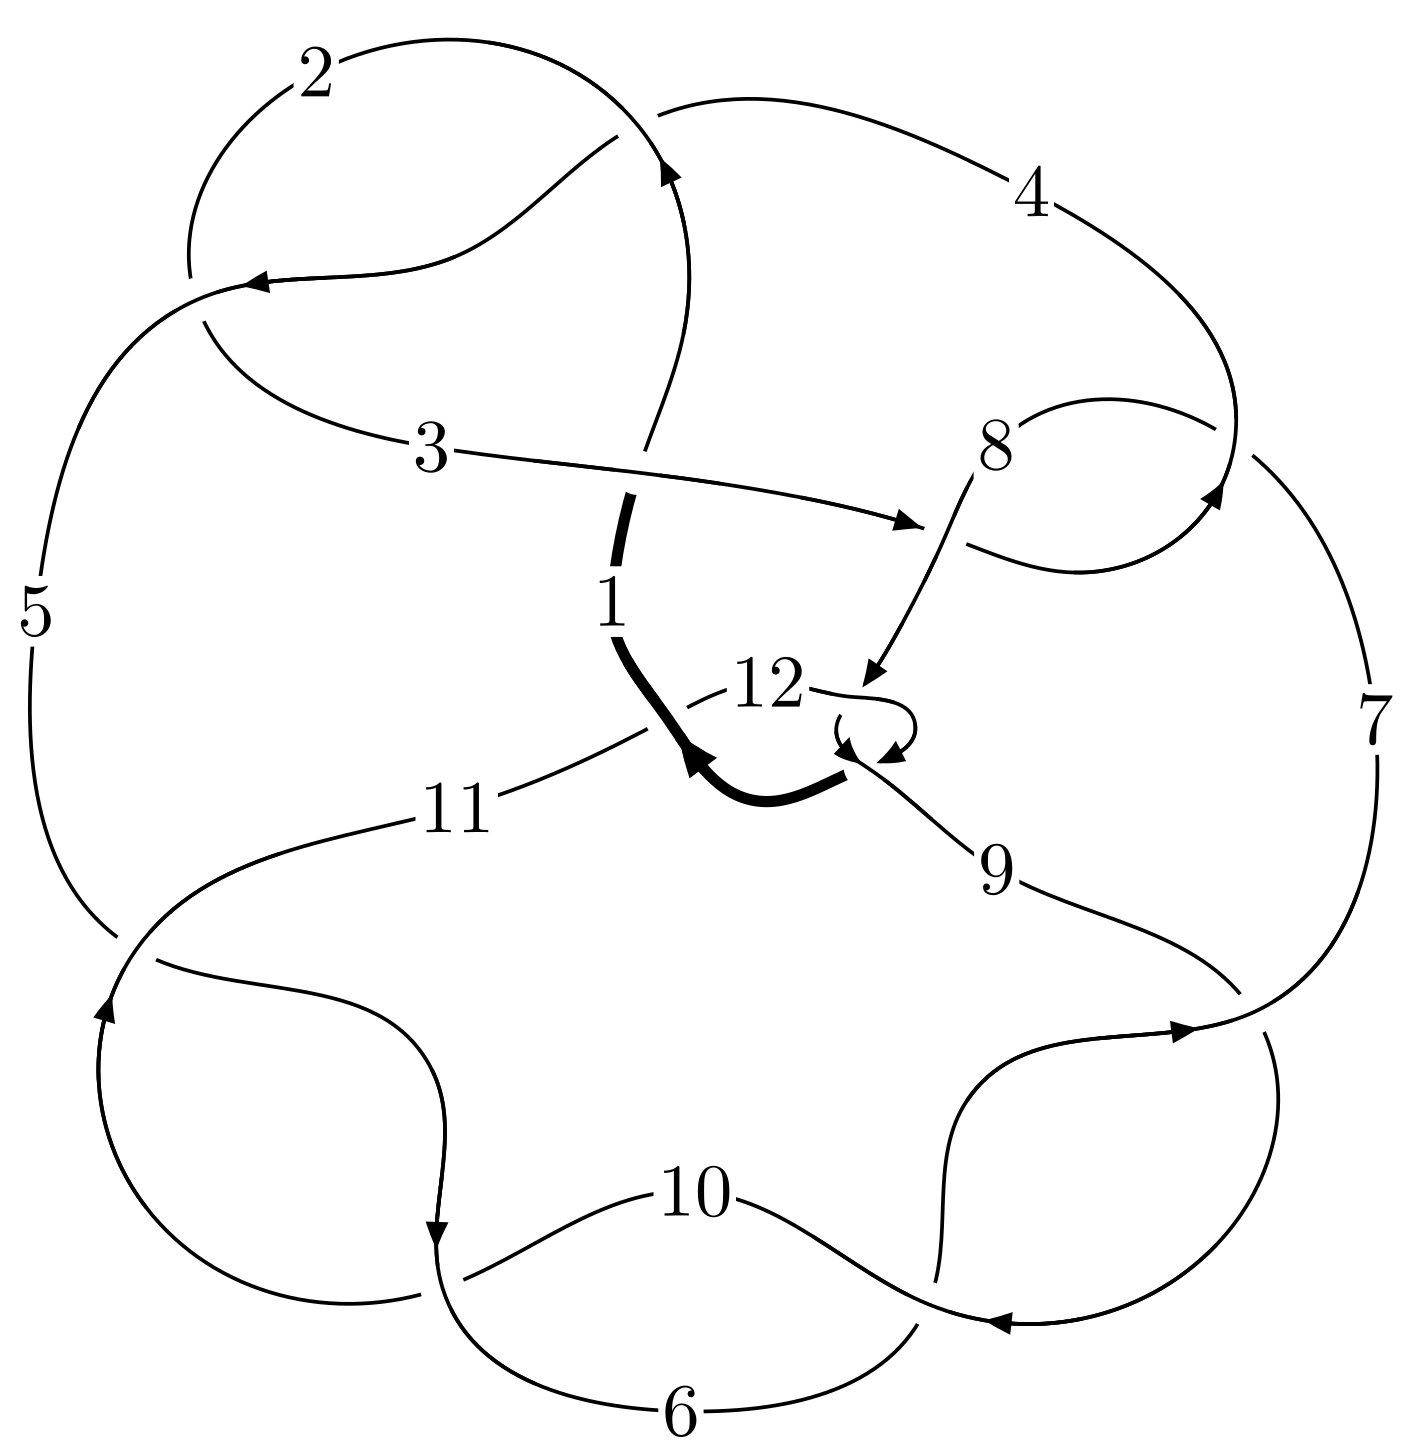
\includegraphics[width=112pt]{../../../GIT/diagram.site/Diagrams/png/910_12a_0109.png}\\
\ \ \ A knot diagram\footnotemark}&
\allowdisplaybreaks
\textbf{Linearized knot diagam} \\
\cline{2-2}
 &
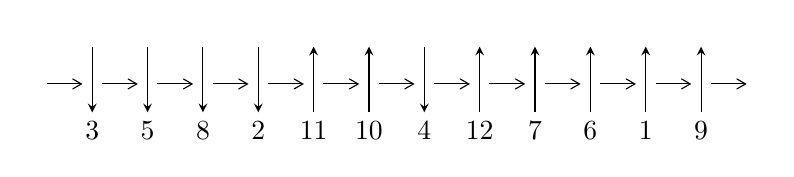
\begin{tikzpicture}[x=20pt, y=17pt]
	% nodes
	\node (C0) at (0, 0) {};
	\node (C1) at (1, 0) {};
	\node (C1U) at (1, +1) {};
	\node (C1D) at (1, -1) {3};

	\node (C2) at (2, 0) {};
	\node (C2U) at (2, +1) {};
	\node (C2D) at (2, -1) {5};

	\node (C3) at (3, 0) {};
	\node (C3U) at (3, +1) {};
	\node (C3D) at (3, -1) {8};

	\node (C4) at (4, 0) {};
	\node (C4U) at (4, +1) {};
	\node (C4D) at (4, -1) {2};

	\node (C5) at (5, 0) {};
	\node (C5U) at (5, +1) {};
	\node (C5D) at (5, -1) {11};

	\node (C6) at (6, 0) {};
	\node (C6U) at (6, +1) {};
	\node (C6D) at (6, -1) {10};

	\node (C7) at (7, 0) {};
	\node (C7U) at (7, +1) {};
	\node (C7D) at (7, -1) {4};

	\node (C8) at (8, 0) {};
	\node (C8U) at (8, +1) {};
	\node (C8D) at (8, -1) {12};

	\node (C9) at (9, 0) {};
	\node (C9U) at (9, +1) {};
	\node (C9D) at (9, -1) {7};

	\node (C10) at (10, 0) {};
	\node (C10U) at (10, +1) {};
	\node (C10D) at (10, -1) {6};

	\node (C11) at (11, 0) {};
	\node (C11U) at (11, +1) {};
	\node (C11D) at (11, -1) {1};

	\node (C12) at (12, 0) {};
	\node (C12U) at (12, +1) {};
	\node (C12D) at (12, -1) {9};
	\node (C13) at (13, 0) {};

	% arrows
	\draw[->,>={angle 60}]
	(C0) edge (C1) (C1) edge (C2) (C2) edge (C3) (C3) edge (C4) (C4) edge (C5) (C5) edge (C6) (C6) edge (C7) (C7) edge (C8) (C8) edge (C9) (C9) edge (C10) (C10) edge (C11) (C11) edge (C12) (C12) edge (C13) ;	\draw[->,>=stealth]
	(C1U) edge (C1D) (C2U) edge (C2D) (C3U) edge (C3D) (C4U) edge (C4D) (C5D) edge (C5U) (C6D) edge (C6U) (C7U) edge (C7D) (C8D) edge (C8U) (C9D) edge (C9U) (C10D) edge (C10U) (C11D) edge (C11U) (C12D) edge (C12U) ;
	\end{tikzpicture} \\
\hhline{~~} \\& 
\textbf{Solving Sequence} \\ \cline{2-2} 
 &
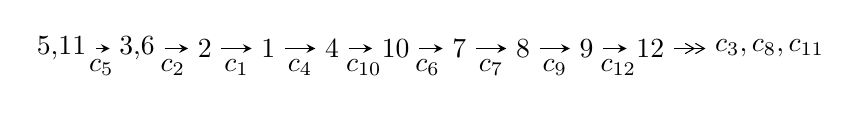
\begin{tikzpicture}[x=23pt, y=7pt]
	% node
	\node (A0) at (-1/8, 0) {5,11};
	\node (A1) at (17/16, 0) {3,6};
	\node (A2) at (17/8, 0) {2};
	\node (A3) at (25/8, 0) {1};
	\node (A4) at (33/8, 0) {4};
	\node (A5) at (41/8, 0) {10};
	\node (A6) at (49/8, 0) {7};
	\node (A7) at (57/8, 0) {8};
	\node (A8) at (65/8, 0) {9};
	\node (A9) at (73/8, 0) {12};
	\node (C1) at (1/2, -1) {$c_{5}$};
	\node (C2) at (13/8, -1) {$c_{2}$};
	\node (C3) at (21/8, -1) {$c_{1}$};
	\node (C4) at (29/8, -1) {$c_{4}$};
	\node (C5) at (37/8, -1) {$c_{10}$};
	\node (C6) at (45/8, -1) {$c_{6}$};
	\node (C7) at (53/8, -1) {$c_{7}$};
	\node (C8) at (61/8, -1) {$c_{9}$};
	\node (C9) at (69/8, -1) {$c_{12}$};
	\node (A10) at (11, 0) {$c_{3},c_{8},c_{11}$};

	% edge
	\draw[->,>=stealth]	
	(A0) edge (A1) (A1) edge (A2) (A2) edge (A3) (A3) edge (A4) (A4) edge (A5) (A5) edge (A6) (A6) edge (A7) (A7) edge (A8) (A8) edge (A9) ;
	\draw[->>,>={angle 60}]	
	(A9) edge (A10);
\end{tikzpicture} \\ 

\end{tabular} \\

\footnotetext{
The image of knot diagram is generated by the software ``\textbf{Draw programme}" developed by Andrew Bartholomew(\url{http://www.layer8.co.uk/maths/draw/index.htm\#Running-draw}), where we modified some parts for our purpose(\url{https://github.com/CATsTAILs/LinksPainter}).
}\phantom \\ \newline 
\centering \textbf{Ideals for irreducible components\footnotemark of $X_{\text{par}}$} 
 
\begin{align*}
I^u_{1}&=\langle 
-5.02927\times10^{100} u^{87}-6.39816\times10^{100} u^{86}+\cdots+3.58918\times10^{101} b+2.49262\times10^{101},\\
\phantom{I^u_{1}}&\phantom{= \langle  }7.25285\times10^{101} u^{87}+1.13095\times10^{102} u^{86}+\cdots+2.15351\times10^{102} a-5.93535\times10^{102},\;u^{88}+2 u^{87}+\cdots-40 u-8\rangle \\
I^u_{2}&=\langle 
b+1,\;-4 u^4-3 u^3-16 u^2+3 a-8 u-10,\;u^5+u^4+4 u^3+3 u^2+3 u+1\rangle \\
I^u_{3}&=\langle 
4 a^2 u-6 a^2-8 a u+17 b+12 a+2 u-20,\;4 a^3+6 a^2 u-8 a^2-2 a u- u-6,\;u^2+2\rangle \\
\\
I^v_{1}&=\langle 
a,\;- v^2+b+3 v+1,\;v^3-2 v^2-3 v-1\rangle \\
\end{align*}
\raggedright * 4 irreducible components of $\dim_{\mathbb{C}}=0$, with total 102 representations.\\
\footnotetext{All coefficients of polynomials are rational numbers. But the coefficients are sometimes approximated in decimal forms when there is not enough margin.}
\newpage
\renewcommand{\arraystretch}{1}
\centering \section*{I. $I^u_{1}= \langle -5.03\times10^{100} u^{87}-6.40\times10^{100} u^{86}+\cdots+3.59\times10^{101} b+2.49\times10^{101},\;7.25\times10^{101} u^{87}+1.13\times10^{102} u^{86}+\cdots+2.15\times10^{102} a-5.94\times10^{102},\;u^{88}+2 u^{87}+\cdots-40 u-8 \rangle$}
\flushleft \textbf{(i) Arc colorings}\\
\begin{tabular}{m{7pt} m{180pt} m{7pt} m{180pt} }
\flushright $a_{5}=$&$\begin{pmatrix}1\\0\end{pmatrix}$ \\
\flushright $a_{11}=$&$\begin{pmatrix}0\\u\end{pmatrix}$ \\
\flushright $a_{3}=$&$\begin{pmatrix}-0.336792 u^{87}-0.525165 u^{86}+\cdots+5.92456 u+2.75613\\0.140123 u^{87}+0.178262 u^{86}+\cdots-3.22318 u-0.694480\end{pmatrix}$ \\
\flushright $a_{6}=$&$\begin{pmatrix}1\\- u^2\end{pmatrix}$ \\
\flushright $a_{2}=$&$\begin{pmatrix}-0.196669 u^{87}-0.346903 u^{86}+\cdots+2.70138 u+2.06165\\0.140123 u^{87}+0.178262 u^{86}+\cdots-3.22318 u-0.694480\end{pmatrix}$ \\
\flushright $a_{1}=$&$\begin{pmatrix}-0.0645847 u^{87}-0.103802 u^{86}+\cdots-3.32912 u-1.32103\\-0.0244135 u^{87}-0.0970148 u^{86}+\cdots+5.00657 u+1.44969\end{pmatrix}$ \\
\flushright $a_{4}=$&$\begin{pmatrix}-0.0540904 u^{87}-0.114055 u^{86}+\cdots-2.19327 u+2.15068\\-0.157753 u^{87}-0.184210 u^{86}+\cdots+5.70265 u+0.193558\end{pmatrix}$ \\
\flushright $a_{10}=$&$\begin{pmatrix}- u\\u^3+u\end{pmatrix}$ \\
\flushright $a_{7}=$&$\begin{pmatrix}u^2+1\\- u^4-2 u^2\end{pmatrix}$ \\
\flushright $a_{8}=$&$\begin{pmatrix}-0.0379577 u^{87}-0.0552205 u^{86}+\cdots+5.05922 u+1.39579\\0.00232376 u^{87}+0.0655726 u^{86}+\cdots-3.90590 u-1.43269\end{pmatrix}$ \\
\flushright $a_{9}=$&$\begin{pmatrix}- u^3-2 u\\u^5+3 u^3+u\end{pmatrix}$ \\
\flushright $a_{12}=$&$\begin{pmatrix}-0.173051 u^{87}-0.352789 u^{86}+\cdots+2.21047 u-0.306496\\-0.0357757 u^{87}-0.0453033 u^{86}+\cdots+2.09794 u+0.712500\end{pmatrix}$\\&\end{tabular}
\flushleft \textbf{(ii) Obstruction class $= -1$}\\~\\
\flushleft \textbf{(iii) Cusp Shapes $= 0.162012 u^{87}+0.0691568 u^{86}+\cdots+10.5321 u-2.78961$}\\~\\
\newpage\renewcommand{\arraystretch}{1}
\flushleft \textbf{(iv) u-Polynomials at the component}\newline \\
\begin{tabular}{m{50pt}|m{274pt}}
Crossings & \hspace{64pt}u-Polynomials at each crossing \\
\hline $$\begin{aligned}c_{1}\end{aligned}$$&$\begin{aligned}
&u^{88}+43 u^{87}+\cdots+5850 u+81
\end{aligned}$\\
\hline $$\begin{aligned}c_{2},c_{4}\end{aligned}$$&$\begin{aligned}
&u^{88}-9 u^{87}+\cdots+12 u+9
\end{aligned}$\\
\hline $$\begin{aligned}c_{3},c_{7}\end{aligned}$$&$\begin{aligned}
&u^{88}+2 u^{87}+\cdots-192 u-288
\end{aligned}$\\
\hline $$\begin{aligned}c_{5},c_{6},c_{9}\\c_{10}\end{aligned}$$&$\begin{aligned}
&u^{88}+2 u^{87}+\cdots-40 u-8
\end{aligned}$\\
\hline $$\begin{aligned}c_{8},c_{12}\end{aligned}$$&$\begin{aligned}
&u^{88}-5 u^{87}+\cdots-525 u+49
\end{aligned}$\\
\hline $$\begin{aligned}c_{11}\end{aligned}$$&$\begin{aligned}
&u^{88}-41 u^{87}+\cdots-246519 u+2401
\end{aligned}$\\
\hline
\end{tabular}\\~\\
\newpage\renewcommand{\arraystretch}{1}
\flushleft \textbf{(v) Riley Polynomials at the component}\newline \\
\begin{tabular}{m{50pt}|m{274pt}}
Crossings & \hspace{64pt}Riley Polynomials at each crossing \\
\hline $$\begin{aligned}c_{1}\end{aligned}$$&$\begin{aligned}
&y^{88}+13 y^{87}+\cdots-26338446 y+6561
\end{aligned}$\\
\hline $$\begin{aligned}c_{2},c_{4}\end{aligned}$$&$\begin{aligned}
&y^{88}-43 y^{87}+\cdots-5850 y+81
\end{aligned}$\\
\hline $$\begin{aligned}c_{3},c_{7}\end{aligned}$$&$\begin{aligned}
&y^{88}+42 y^{87}+\cdots+59904 y+82944
\end{aligned}$\\
\hline $$\begin{aligned}c_{5},c_{6},c_{9}\\c_{10}\end{aligned}$$&$\begin{aligned}
&y^{88}+104 y^{87}+\cdots-448 y+64
\end{aligned}$\\
\hline $$\begin{aligned}c_{8},c_{12}\end{aligned}$$&$\begin{aligned}
&y^{88}-41 y^{87}+\cdots-246519 y+2401
\end{aligned}$\\
\hline $$\begin{aligned}c_{11}\end{aligned}$$&$\begin{aligned}
&y^{88}+23 y^{87}+\cdots-42416044391 y+5764801
\end{aligned}$\\
\hline
\end{tabular}\\~\\
\newpage\flushleft \textbf{(vi) Complex Volumes and Cusp Shapes}
$$\begin{array}{c|c|c}  
\text{Solutions to }I^u_{1}& \I (\text{vol} + \sqrt{-1}CS) & \text{Cusp shape}\\
 \hline 
\begin{aligned}
u &= \phantom{-}0.544232 + 0.801981 I \\
a &= \phantom{-}0.45727 + 1.70633 I \\
b &= \phantom{-}1.122770 - 0.558543 I\end{aligned}
 & -1.95733 + 7.43628 I & \phantom{-0.000000 } 0 \\ \hline\begin{aligned}
u &= \phantom{-}0.544232 - 0.801981 I \\
a &= \phantom{-}0.45727 - 1.70633 I \\
b &= \phantom{-}1.122770 + 0.558543 I\end{aligned}
 & -1.95733 - 7.43628 I & \phantom{-0.000000 } 0 \\ \hline\begin{aligned}
u &= -0.639200 + 0.724714 I \\
a &= \phantom{-}0.19749 - 2.03333 I \\
b &= \phantom{-}1.172430 + 0.616645 I\end{aligned}
 & \phantom{-}0.25275 - 13.11110 I & \phantom{-0.000000 } 0 \\ \hline\begin{aligned}
u &= -0.639200 - 0.724714 I \\
a &= \phantom{-}0.19749 + 2.03333 I \\
b &= \phantom{-}1.172430 - 0.616645 I\end{aligned}
 & \phantom{-}0.25275 + 13.11110 I & \phantom{-0.000000 } 0 \\ \hline\begin{aligned}
u &= \phantom{-}0.425748 + 0.993580 I \\
a &= \phantom{-}0.064085 + 0.159980 I \\
b &= \phantom{-}0.957165 + 0.380322 I\end{aligned}
 & -3.21813 + 0.79813 I & \phantom{-0.000000 } 0 \\ \hline\begin{aligned}
u &= \phantom{-}0.425748 - 0.993580 I \\
a &= \phantom{-}0.064085 - 0.159980 I \\
b &= \phantom{-}0.957165 - 0.380322 I\end{aligned}
 & -3.21813 - 0.79813 I & \phantom{-0.000000 } 0 \\ \hline\begin{aligned}
u &= -0.589414 + 0.668596 I \\
a &= -0.901108 + 0.955267 I \\
b &= \phantom{-}0.339571 - 0.905352 I\end{aligned}
 & \phantom{-}2.77273 - 7.53893 I & \phantom{-0.000000 } 0 \\ \hline\begin{aligned}
u &= -0.589414 - 0.668596 I \\
a &= -0.901108 - 0.955267 I \\
b &= \phantom{-}0.339571 + 0.905352 I\end{aligned}
 & \phantom{-}2.77273 + 7.53893 I & \phantom{-0.000000 } 0 \\ \hline\begin{aligned}
u &= \phantom{-}0.521144 + 0.708575 I \\
a &= \phantom{-}0.09047 - 2.35621 I \\
b &= -1.035090 + 0.541644 I\end{aligned}
 & -1.93302 + 6.75586 I & \phantom{-0.000000 } 0 \\ \hline\begin{aligned}
u &= \phantom{-}0.521144 - 0.708575 I \\
a &= \phantom{-}0.09047 + 2.35621 I \\
b &= -1.035090 - 0.541644 I\end{aligned}
 & -1.93302 - 6.75586 I & \phantom{-0.000000 } 0\\
 \hline 
 \end{array}$$\newpage$$\begin{array}{c|c|c}  
\text{Solutions to }I^u_{1}& \I (\text{vol} + \sqrt{-1}CS) & \text{Cusp shape}\\
 \hline 
\begin{aligned}
u &= -0.454359 + 0.719803 I \\
a &= \phantom{-}0.108044 + 0.326009 I \\
b &= -1.287330 + 0.187629 I\end{aligned}
 & -2.77018 - 4.12176 I & \phantom{-0.000000 -}0. + 7.16112 I \\ \hline\begin{aligned}
u &= -0.454359 - 0.719803 I \\
a &= \phantom{-}0.108044 - 0.326009 I \\
b &= -1.287330 - 0.187629 I\end{aligned}
 & -2.77018 + 4.12176 I & \phantom{-0.000000 } 0. - 7.16112 I \\ \hline\begin{aligned}
u &= \phantom{-}0.189661 + 0.796762 I \\
a &= -0.421221 + 0.469754 I \\
b &= -1.170030 - 0.256475 I\end{aligned}
 & -4.00054 - 0.43094 I & -4.62005 - 1.23771 I \\ \hline\begin{aligned}
u &= \phantom{-}0.189661 - 0.796762 I \\
a &= -0.421221 - 0.469754 I \\
b &= -1.170030 + 0.256475 I\end{aligned}
 & -4.00054 + 0.43094 I & -4.62005 + 1.23771 I \\ \hline\begin{aligned}
u &= \phantom{-}0.476204 + 0.665286 I \\
a &= -0.583867 - 0.579072 I \\
b &= \phantom{-}0.308494 + 0.733628 I\end{aligned}
 & \phantom{-}0.39849 + 2.53090 I & \phantom{-}2.00000 - 3.36549 I \\ \hline\begin{aligned}
u &= \phantom{-}0.476204 - 0.665286 I \\
a &= -0.583867 + 0.579072 I \\
b &= \phantom{-}0.308494 - 0.733628 I\end{aligned}
 & \phantom{-}0.39849 - 2.53090 I & \phantom{-}2.00000 + 3.36549 I \\ \hline\begin{aligned}
u &= -0.325850 + 0.749057 I \\
a &= -0.33571 + 2.12266 I \\
b &= -1.063440 - 0.409718 I\end{aligned}
 & -3.62884 - 1.93734 I & -4.67467 + 2.40265 I \\ \hline\begin{aligned}
u &= -0.325850 - 0.749057 I \\
a &= -0.33571 - 2.12266 I \\
b &= -1.063440 + 0.409718 I\end{aligned}
 & -3.62884 + 1.93734 I & -4.67467 - 2.40265 I \\ \hline\begin{aligned}
u &= -0.764680 + 0.260523 I \\
a &= -1.01456 + 1.01023 I \\
b &= \phantom{-}1.121010 - 0.587805 I\end{aligned}
 & \phantom{-}1.64540 + 8.43286 I & \phantom{-}2.93830 - 6.25674 I \\ \hline\begin{aligned}
u &= -0.764680 - 0.260523 I \\
a &= -1.01456 - 1.01023 I \\
b &= \phantom{-}1.121010 + 0.587805 I\end{aligned}
 & \phantom{-}1.64540 - 8.43286 I & \phantom{-}2.93830 + 6.25674 I\\
 \hline 
 \end{array}$$\newpage$$\begin{array}{c|c|c}  
\text{Solutions to }I^u_{1}& \I (\text{vol} + \sqrt{-1}CS) & \text{Cusp shape}\\
 \hline 
\begin{aligned}
u &= \phantom{-}0.209318 + 1.208190 I \\
a &= \phantom{-}0.464577 + 0.697157 I \\
b &= \phantom{-}0.852854 - 0.450479 I\end{aligned}
 & -3.00819 + 4.00876 I & \phantom{-0.000000 } 0 \\ \hline\begin{aligned}
u &= \phantom{-}0.209318 - 1.208190 I \\
a &= \phantom{-}0.464577 - 0.697157 I \\
b &= \phantom{-}0.852854 + 0.450479 I\end{aligned}
 & -3.00819 - 4.00876 I & \phantom{-0.000000 } 0 \\ \hline\begin{aligned}
u &= \phantom{-}0.367904 + 0.650557 I \\
a &= \phantom{-}1.28515 + 1.07932 I \\
b &= -0.523066 - 0.570388 I\end{aligned}
 & -0.39958 + 2.25212 I & \phantom{-}1.06124 - 3.79280 I \\ \hline\begin{aligned}
u &= \phantom{-}0.367904 - 0.650557 I \\
a &= \phantom{-}1.28515 - 1.07932 I \\
b &= -0.523066 + 0.570388 I\end{aligned}
 & -0.39958 - 2.25212 I & \phantom{-}1.06124 + 3.79280 I \\ \hline\begin{aligned}
u &= -0.295855 + 1.218520 I \\
a &= \phantom{-}0.010588 + 0.192785 I \\
b &= \phantom{-}1.046980 - 0.516890 I\end{aligned}
 & -3.02122 + 4.63137 I & \phantom{-0.000000 } 0 \\ \hline\begin{aligned}
u &= -0.295855 - 1.218520 I \\
a &= \phantom{-}0.010588 - 0.192785 I \\
b &= \phantom{-}1.046980 + 0.516890 I\end{aligned}
 & -3.02122 - 4.63137 I & \phantom{-0.000000 } 0 \\ \hline\begin{aligned}
u &= \phantom{-}0.736276 + 0.098653 I \\
a &= -0.817831 - 0.970106 I \\
b &= \phantom{-}1.025650 + 0.511792 I\end{aligned}
 & \phantom{-}0.17226 - 3.17277 I & \phantom{-}1.85523 + 2.82339 I \\ \hline\begin{aligned}
u &= \phantom{-}0.736276 - 0.098653 I \\
a &= -0.817831 + 0.970106 I \\
b &= \phantom{-}1.025650 - 0.511792 I\end{aligned}
 & \phantom{-}0.17226 + 3.17277 I & \phantom{-}1.85523 - 2.82339 I \\ \hline\begin{aligned}
u &= -0.674195 + 0.305262 I \\
a &= \phantom{-}0.11126 - 1.73615 I \\
b &= \phantom{-}0.372533 + 0.786143 I\end{aligned}
 & \phantom{-}3.86256 + 3.27144 I & \phantom{-}6.73775 - 1.69394 I \\ \hline\begin{aligned}
u &= -0.674195 - 0.305262 I \\
a &= \phantom{-}0.11126 + 1.73615 I \\
b &= \phantom{-}0.372533 - 0.786143 I\end{aligned}
 & \phantom{-}3.86256 - 3.27144 I & \phantom{-}6.73775 + 1.69394 I\\
 \hline 
 \end{array}$$\newpage$$\begin{array}{c|c|c}  
\text{Solutions to }I^u_{1}& \I (\text{vol} + \sqrt{-1}CS) & \text{Cusp shape}\\
 \hline 
\begin{aligned}
u &= \phantom{-}0.034179 + 0.718127 I \\
a &= \phantom{-}0.764549 - 0.742243 I \\
b &= -0.184555 + 0.451760 I\end{aligned}
 & -1.22278 + 1.55214 I & -0.78508 - 5.01782 I \\ \hline\begin{aligned}
u &= \phantom{-}0.034179 - 0.718127 I \\
a &= \phantom{-}0.764549 + 0.742243 I \\
b &= -0.184555 - 0.451760 I\end{aligned}
 & -1.22278 - 1.55214 I & -0.78508 + 5.01782 I \\ \hline\begin{aligned}
u &= -0.317676 + 0.640571 I \\
a &= \phantom{-}1.74066 - 1.75496 I \\
b &= \phantom{-}1.001370 + 0.622107 I\end{aligned}
 & \phantom{-}3.82065 - 4.46578 I & \phantom{-}2.93072 + 6.78920 I \\ \hline\begin{aligned}
u &= -0.317676 - 0.640571 I \\
a &= \phantom{-}1.74066 + 1.75496 I \\
b &= \phantom{-}1.001370 - 0.622107 I\end{aligned}
 & \phantom{-}3.82065 + 4.46578 I & \phantom{-}2.93072 - 6.78920 I \\ \hline\begin{aligned}
u &= -0.440566 + 0.518571 I \\
a &= -1.302340 - 0.305908 I \\
b &= \phantom{-}0.590084 - 0.713658 I\end{aligned}
 & \phantom{-}5.03768 + 0.64765 I & \phantom{-}6.53702 + 1.45121 I \\ \hline\begin{aligned}
u &= -0.440566 - 0.518571 I \\
a &= -1.302340 + 0.305908 I \\
b &= \phantom{-}0.590084 + 0.713658 I\end{aligned}
 & \phantom{-}5.03768 - 0.64765 I & \phantom{-}6.53702 - 1.45121 I \\ \hline\begin{aligned}
u &= \phantom{-}0.617215 + 0.203807 I \\
a &= \phantom{-}1.68584 + 1.45481 I \\
b &= -1.002130 - 0.427316 I\end{aligned}
 & -0.43590 - 2.88040 I & \phantom{-}1.88878 + 2.99748 I \\ \hline\begin{aligned}
u &= \phantom{-}0.617215 - 0.203807 I \\
a &= \phantom{-}1.68584 - 1.45481 I \\
b &= -1.002130 + 0.427316 I\end{aligned}
 & -0.43590 + 2.88040 I & \phantom{-}1.88878 - 2.99748 I \\ \hline\begin{aligned}
u &= \phantom{-}0.594706 + 0.256396 I \\
a &= -0.073072 + 1.290030 I \\
b &= \phantom{-}0.553067 - 0.541679 I\end{aligned}
 & \phantom{-}1.61593 + 1.10166 I & \phantom{-}4.49842 - 4.17125 I \\ \hline\begin{aligned}
u &= \phantom{-}0.594706 - 0.256396 I \\
a &= -0.073072 - 1.290030 I \\
b &= \phantom{-}0.553067 + 0.541679 I\end{aligned}
 & \phantom{-}1.61593 - 1.10166 I & \phantom{-}4.49842 + 4.17125 I\\
 \hline 
 \end{array}$$\newpage$$\begin{array}{c|c|c}  
\text{Solutions to }I^u_{1}& \I (\text{vol} + \sqrt{-1}CS) & \text{Cusp shape}\\
 \hline 
\begin{aligned}
u &= \phantom{-}0.037223 + 1.354310 I \\
a &= \phantom{-}1.29186 + 1.33974 I \\
b &= -0.935436 - 0.213125 I\end{aligned}
 & -4.84743 - 0.66518 I & \phantom{-0.000000 } 0 \\ \hline\begin{aligned}
u &= \phantom{-}0.037223 - 1.354310 I \\
a &= \phantom{-}1.29186 - 1.33974 I \\
b &= -0.935436 + 0.213125 I\end{aligned}
 & -4.84743 + 0.66518 I & \phantom{-0.000000 } 0 \\ \hline\begin{aligned}
u &= -0.184148 + 1.365040 I \\
a &= \phantom{-}0.520576 - 0.880021 I \\
b &= \phantom{-}0.481633 + 0.586417 I\end{aligned}
 & -1.360140 + 0.220167 I & \phantom{-0.000000 } 0 \\ \hline\begin{aligned}
u &= -0.184148 - 1.365040 I \\
a &= \phantom{-}0.520576 + 0.880021 I \\
b &= \phantom{-}0.481633 - 0.586417 I\end{aligned}
 & -1.360140 - 0.220167 I & \phantom{-0.000000 } 0 \\ \hline\begin{aligned}
u &= -0.396296 + 0.432190 I \\
a &= -0.49246 - 1.73630 I \\
b &= \phantom{-}0.740300 + 0.830855 I\end{aligned}
 & \phantom{-}5.31869 - 3.65991 I & \phantom{-}6.10187 + 9.13654 I \\ \hline\begin{aligned}
u &= -0.396296 - 0.432190 I \\
a &= -0.49246 + 1.73630 I \\
b &= \phantom{-}0.740300 - 0.830855 I\end{aligned}
 & \phantom{-}5.31869 + 3.65991 I & \phantom{-}6.10187 - 9.13654 I \\ \hline\begin{aligned}
u &= -0.542158 + 0.117917 I \\
a &= \phantom{-}1.37098 + 1.98919 I \\
b &= -1.142410 - 0.181756 I\end{aligned}
 & -1.021790 + 0.705294 I & \phantom{-}3.49954 - 4.37901 I \\ \hline\begin{aligned}
u &= -0.542158 - 0.117917 I \\
a &= \phantom{-}1.37098 - 1.98919 I \\
b &= -1.142410 + 0.181756 I\end{aligned}
 & -1.021790 - 0.705294 I & \phantom{-}3.49954 + 4.37901 I \\ \hline\begin{aligned}
u &= \phantom{-}0.03018 + 1.52198 I \\
a &= -2.04233 - 1.47340 I \\
b &= -1.045690 + 0.315482 I\end{aligned}
 & -5.53360 + 1.03148 I & \phantom{-0.000000 } 0 \\ \hline\begin{aligned}
u &= \phantom{-}0.03018 - 1.52198 I \\
a &= -2.04233 + 1.47340 I \\
b &= -1.045690 - 0.315482 I\end{aligned}
 & -5.53360 - 1.03148 I & \phantom{-0.000000 } 0\\
 \hline 
 \end{array}$$\newpage$$\begin{array}{c|c|c}  
\text{Solutions to }I^u_{1}& \I (\text{vol} + \sqrt{-1}CS) & \text{Cusp shape}\\
 \hline 
\begin{aligned}
u &= -0.04131 + 1.52824 I \\
a &= -0.061906 + 0.831333 I \\
b &= \phantom{-}0.962138 - 0.868668 I\end{aligned}
 & -1.82017 + 1.37348 I & \phantom{-0.000000 } 0 \\ \hline\begin{aligned}
u &= -0.04131 - 1.52824 I \\
a &= -0.061906 - 0.831333 I \\
b &= \phantom{-}0.962138 + 0.868668 I\end{aligned}
 & -1.82017 - 1.37348 I & \phantom{-0.000000 } 0 \\ \hline\begin{aligned}
u &= -0.11035 + 1.53163 I \\
a &= -0.149288 - 0.272362 I \\
b &= \phantom{-}0.368366 - 0.654466 I\end{aligned}
 & -1.82032 - 1.29038 I & \phantom{-0.000000 } 0 \\ \hline\begin{aligned}
u &= -0.11035 - 1.53163 I \\
a &= -0.149288 + 0.272362 I \\
b &= \phantom{-}0.368366 + 0.654466 I\end{aligned}
 & -1.82032 + 1.29038 I & \phantom{-0.000000 } 0 \\ \hline\begin{aligned}
u &= -0.08013 + 1.53516 I \\
a &= \phantom{-}0.071720 - 0.991753 I \\
b &= \phantom{-}0.806978 + 0.935865 I\end{aligned}
 & -1.34895 - 5.18025 I & \phantom{-0.000000 } 0 \\ \hline\begin{aligned}
u &= -0.08013 - 1.53516 I \\
a &= \phantom{-}0.071720 + 0.991753 I \\
b &= \phantom{-}0.806978 - 0.935865 I\end{aligned}
 & -1.34895 + 5.18025 I & \phantom{-0.000000 } 0 \\ \hline\begin{aligned}
u &= -0.262252 + 0.372162 I \\
a &= -0.93452 + 1.46801 I \\
b &= \phantom{-}0.950259 - 0.771844 I\end{aligned}
 & \phantom{-}4.71038 + 2.27505 I & \phantom{-}2.87495 + 6.92818 I \\ \hline\begin{aligned}
u &= -0.262252 - 0.372162 I \\
a &= -0.93452 - 1.46801 I \\
b &= \phantom{-}0.950259 + 0.771844 I\end{aligned}
 & \phantom{-}4.71038 - 2.27505 I & \phantom{-}2.87495 - 6.92818 I \\ \hline\begin{aligned}
u &= \phantom{-}0.280491 + 0.286926 I \\
a &= -0.03250 - 5.56793 I \\
b &= -0.763793 + 0.248992 I\end{aligned}
 & \phantom{-}0.742521 + 0.263079 I & \phantom{-}1.89432 - 10.85247 I \\ \hline\begin{aligned}
u &= \phantom{-}0.280491 - 0.286926 I \\
a &= -0.03250 + 5.56793 I \\
b &= -0.763793 - 0.248992 I\end{aligned}
 & \phantom{-}0.742521 - 0.263079 I & \phantom{-}1.89432 + 10.85247 I\\
 \hline 
 \end{array}$$\newpage$$\begin{array}{c|c|c}  
\text{Solutions to }I^u_{1}& \I (\text{vol} + \sqrt{-1}CS) & \text{Cusp shape}\\
 \hline 
\begin{aligned}
u &= \phantom{-}0.10435 + 1.59638 I \\
a &= \phantom{-}0.597044 + 0.707359 I \\
b &= -0.520082 - 0.766678 I\end{aligned}
 & -8.09429 + 3.99340 I & \phantom{-0.000000 } 0 \\ \hline\begin{aligned}
u &= \phantom{-}0.10435 - 1.59638 I \\
a &= \phantom{-}0.597044 - 0.707359 I \\
b &= -0.520082 + 0.766678 I\end{aligned}
 & -8.09429 - 3.99340 I & \phantom{-0.000000 } 0 \\ \hline\begin{aligned}
u &= \phantom{-}0.13215 + 1.59776 I \\
a &= -0.287968 - 0.352186 I \\
b &= \phantom{-}0.216304 + 0.908312 I\end{aligned}
 & -7.29353 + 4.75365 I & \phantom{-0.000000 } 0 \\ \hline\begin{aligned}
u &= \phantom{-}0.13215 - 1.59776 I \\
a &= -0.287968 + 0.352186 I \\
b &= \phantom{-}0.216304 - 0.908312 I\end{aligned}
 & -7.29353 - 4.75365 I & \phantom{-0.000000 } 0 \\ \hline\begin{aligned}
u &= -0.09037 + 1.60143 I \\
a &= \phantom{-}1.44988 - 0.84143 I \\
b &= \phantom{-}1.091120 + 0.543357 I\end{aligned}
 & -3.91219 - 5.96968 I & \phantom{-0.000000 } 0 \\ \hline\begin{aligned}
u &= -0.09037 - 1.60143 I \\
a &= \phantom{-}1.44988 + 0.84143 I \\
b &= \phantom{-}1.091120 - 0.543357 I\end{aligned}
 & -3.91219 + 5.96968 I & \phantom{-0.000000 } 0 \\ \hline\begin{aligned}
u &= -0.17781 + 1.59504 I \\
a &= -0.539469 + 0.440389 I \\
b &= \phantom{-}0.314437 - 0.996490 I\end{aligned}
 & -4.83782 - 10.38830 I & \phantom{-0.000000 } 0 \\ \hline\begin{aligned}
u &= -0.17781 - 1.59504 I \\
a &= -0.539469 - 0.440389 I \\
b &= \phantom{-}0.314437 + 0.996490 I\end{aligned}
 & -4.83782 + 10.38830 I & \phantom{-0.000000 } 0 \\ \hline\begin{aligned}
u &= -0.02758 + 1.60517 I \\
a &= \phantom{-}0.427081 - 0.575629 I \\
b &= -0.297892 + 0.763089 I\end{aligned}
 & -9.20407 + 1.33304 I & \phantom{-0.000000 } 0 \\ \hline\begin{aligned}
u &= -0.02758 - 1.60517 I \\
a &= \phantom{-}0.427081 + 0.575629 I \\
b &= -0.297892 - 0.763089 I\end{aligned}
 & -9.20407 - 1.33304 I & \phantom{-0.000000 } 0\\
 \hline 
 \end{array}$$\newpage$$\begin{array}{c|c|c}  
\text{Solutions to }I^u_{1}& \I (\text{vol} + \sqrt{-1}CS) & \text{Cusp shape}\\
 \hline 
\begin{aligned}
u &= \phantom{-}0.15240 + 1.60919 I \\
a &= -0.50275 - 1.61138 I \\
b &= -1.078540 + 0.619975 I\end{aligned}
 & -9.79087 + 9.27121 I & \phantom{-0.000000 } 0 \\ \hline\begin{aligned}
u &= \phantom{-}0.15240 - 1.60919 I \\
a &= -0.50275 + 1.61138 I \\
b &= -1.078540 - 0.619975 I\end{aligned}
 & -9.79087 - 9.27121 I & \phantom{-0.000000 } 0 \\ \hline\begin{aligned}
u &= -0.13042 + 1.61198 I \\
a &= -0.665204 + 0.200185 I \\
b &= -1.377650 + 0.211486 I\end{aligned}
 & -10.71360 - 6.30775 I & \phantom{-0.000000 } 0 \\ \hline\begin{aligned}
u &= -0.13042 - 1.61198 I \\
a &= -0.665204 - 0.200185 I \\
b &= -1.377650 - 0.211486 I\end{aligned}
 & -10.71360 + 6.30775 I & \phantom{-0.000000 } 0 \\ \hline\begin{aligned}
u &= -0.09497 + 1.61734 I \\
a &= -0.71777 + 1.37284 I \\
b &= -1.140320 - 0.532443 I\end{aligned}
 & -11.73680 - 3.53945 I & \phantom{-0.000000 } 0 \\ \hline\begin{aligned}
u &= -0.09497 - 1.61734 I \\
a &= -0.71777 - 1.37284 I \\
b &= -1.140320 + 0.532443 I\end{aligned}
 & -11.73680 + 3.53945 I & \phantom{-0.000000 } 0 \\ \hline\begin{aligned}
u &= \phantom{-}0.378309\phantom{ +0.000000I} \\
a &= \phantom{-}1.75496\phantom{ +0.000000I} \\
b &= -0.125481\phantom{ +0.000000I}\end{aligned}
 & \phantom{-}1.01782\phantom{ +0.000000I} & \phantom{-}11.4040\phantom{ +0.000000I} \\ \hline\begin{aligned}
u &= \phantom{-}0.06578 + 1.62137 I \\
a &= -0.858345 + 0.218227 I \\
b &= -1.316490 - 0.299557 I\end{aligned}
 & -12.27180 + 0.62227 I & \phantom{-0.000000 } 0 \\ \hline\begin{aligned}
u &= \phantom{-}0.06578 - 1.62137 I \\
a &= -0.858345 - 0.218227 I \\
b &= -1.316490 + 0.299557 I\end{aligned}
 & -12.27180 - 0.62227 I & \phantom{-0.000000 } 0 \\ \hline\begin{aligned}
u &= -0.19926 + 1.61688 I \\
a &= \phantom{-}0.81358 - 1.44253 I \\
b &= \phantom{-}1.218140 + 0.634975 I\end{aligned}
 & -7.6180 - 16.2777 I & \phantom{-0.000000 } 0\\
 \hline 
 \end{array}$$\newpage$$\begin{array}{c|c|c}  
\text{Solutions to }I^u_{1}& \I (\text{vol} + \sqrt{-1}CS) & \text{Cusp shape}\\
 \hline 
\begin{aligned}
u &= -0.19926 - 1.61688 I \\
a &= \phantom{-}0.81358 + 1.44253 I \\
b &= \phantom{-}1.218140 - 0.634975 I\end{aligned}
 & -7.6180 + 16.2777 I & \phantom{-0.000000 } 0 \\ \hline\begin{aligned}
u &= \phantom{-}0.15988 + 1.63933 I \\
a &= \phantom{-}0.89920 + 1.16202 I \\
b &= \phantom{-}1.204800 - 0.573189 I\end{aligned}
 & -10.2649 + 10.1230 I & \phantom{-0.000000 } 0 \\ \hline\begin{aligned}
u &= \phantom{-}0.15988 - 1.63933 I \\
a &= \phantom{-}0.89920 - 1.16202 I \\
b &= \phantom{-}1.204800 + 0.573189 I\end{aligned}
 & -10.2649 - 10.1230 I & \phantom{-0.000000 } 0 \\ \hline\begin{aligned}
u &= -0.00661 + 1.70566 I \\
a &= \phantom{-}0.785461 + 0.141099 I \\
b &= \phantom{-}1.083240 - 0.305675 I\end{aligned}
 & -13.33910 + 4.11275 I & \phantom{-0.000000 } 0 \\ \hline\begin{aligned}
u &= -0.00661 - 1.70566 I \\
a &= \phantom{-}0.785461 - 0.141099 I \\
b &= \phantom{-}1.083240 + 0.305675 I\end{aligned}
 & -13.33910 - 4.11275 I & \phantom{-0.000000 } 0 \\ \hline\begin{aligned}
u &= \phantom{-}0.09125 + 1.70355 I \\
a &= \phantom{-}0.686106 + 0.124440 I \\
b &= \phantom{-}0.983741 + 0.219632 I\end{aligned}
 & -12.68530 + 2.74860 I & \phantom{-0.000000 } 0 \\ \hline\begin{aligned}
u &= \phantom{-}0.09125 - 1.70355 I \\
a &= \phantom{-}0.686106 - 0.124440 I \\
b &= \phantom{-}0.983741 - 0.219632 I\end{aligned}
 & -12.68530 - 2.74860 I & \phantom{-0.000000 } 0 \\ \hline\begin{aligned}
u &= -0.227971\phantom{ +0.000000I} \\
a &= \phantom{-}3.59324\phantom{ +0.000000I} \\
b &= -0.877499\phantom{ +0.000000I}\end{aligned}
 & -1.26625\phantom{ +0.000000I} & -9.48720\phantom{ +0.000000I}\\
 \hline 
 \end{array}$$\newpage\newpage\renewcommand{\arraystretch}{1}
\centering \section*{II. $I^u_{2}= \langle b+1,\;-4 u^4-3 u^3-16 u^2+3 a-8 u-10,\;u^5+u^4+4 u^3+3 u^2+3 u+1 \rangle$}
\flushleft \textbf{(i) Arc colorings}\\
\begin{tabular}{m{7pt} m{180pt} m{7pt} m{180pt} }
\flushright $a_{5}=$&$\begin{pmatrix}1\\0\end{pmatrix}$ \\
\flushright $a_{11}=$&$\begin{pmatrix}0\\u\end{pmatrix}$ \\
\flushright $a_{3}=$&$\begin{pmatrix}\frac{4}{3} u^4+u^3+\frac{16}{3} u^2+\frac{8}{3} u+\frac{10}{3}\\-1\end{pmatrix}$ \\
\flushright $a_{6}=$&$\begin{pmatrix}1\\- u^2\end{pmatrix}$ \\
\flushright $a_{2}=$&$\begin{pmatrix}\frac{4}{3} u^4+u^3+\frac{16}{3} u^2+\frac{8}{3} u+\frac{7}{3}\\-1\end{pmatrix}$ \\
\flushright $a_{1}=$&$\begin{pmatrix}-1\\0\end{pmatrix}$ \\
\flushright $a_{4}=$&$\begin{pmatrix}\frac{4}{3} u^4+u^3+\frac{16}{3} u^2+\frac{8}{3} u+\frac{10}{3}\\-1\end{pmatrix}$ \\
\flushright $a_{10}=$&$\begin{pmatrix}- u\\u^3+u\end{pmatrix}$ \\
\flushright $a_{7}=$&$\begin{pmatrix}u^2+1\\- u^4-2 u^2\end{pmatrix}$ \\
\flushright $a_{8}=$&$\begin{pmatrix}u^2+1\\- u^4-2 u^2\end{pmatrix}$ \\
\flushright $a_{9}=$&$\begin{pmatrix}- u^3-2 u\\- u^4- u^3-3 u^2-2 u-1\end{pmatrix}$ \\
\flushright $a_{12}=$&$\begin{pmatrix}u\\u\end{pmatrix}$\\&\end{tabular}
\flushleft \textbf{(ii) Obstruction class $= 1$}\\~\\
\flushleft \textbf{(iii) Cusp Shapes $= \frac{58}{9} u^4+\frac{13}{3} u^3+\frac{211}{9} u^2+\frac{128}{9} u+\frac{115}{9}$}\\~\\
\newpage\renewcommand{\arraystretch}{1}
\flushleft \textbf{(iv) u-Polynomials at the component}\newline \\
\begin{tabular}{m{50pt}|m{274pt}}
Crossings & \hspace{64pt}u-Polynomials at each crossing \\
\hline $$\begin{aligned}c_{1},c_{2}\end{aligned}$$&$\begin{aligned}
&(u-1)^5
\end{aligned}$\\
\hline $$\begin{aligned}c_{3},c_{7}\end{aligned}$$&$\begin{aligned}
&u^5
\end{aligned}$\\
\hline $$\begin{aligned}c_{4}\end{aligned}$$&$\begin{aligned}
&(u+1)^5
\end{aligned}$\\
\hline $$\begin{aligned}c_{5},c_{6},c_{11}\end{aligned}$$&$\begin{aligned}
&u^5+u^4+4 u^3+3 u^2+3 u+1
\end{aligned}$\\
\hline $$\begin{aligned}c_{8}\end{aligned}$$&$\begin{aligned}
&u^5+u^4- u^2+u+1
\end{aligned}$\\
\hline $$\begin{aligned}c_{9},c_{10}\end{aligned}$$&$\begin{aligned}
&u^5- u^4+4 u^3-3 u^2+3 u-1
\end{aligned}$\\
\hline $$\begin{aligned}c_{12}\end{aligned}$$&$\begin{aligned}
&u^5- u^4+u^2+u-1
\end{aligned}$\\
\hline
\end{tabular}\\~\\
\newpage\renewcommand{\arraystretch}{1}
\flushleft \textbf{(v) Riley Polynomials at the component}\newline \\
\begin{tabular}{m{50pt}|m{274pt}}
Crossings & \hspace{64pt}Riley Polynomials at each crossing \\
\hline $$\begin{aligned}c_{1},c_{2},c_{4}\end{aligned}$$&$\begin{aligned}
&(y-1)^5
\end{aligned}$\\
\hline $$\begin{aligned}c_{3},c_{7}\end{aligned}$$&$\begin{aligned}
&y^5
\end{aligned}$\\
\hline $$\begin{aligned}c_{5},c_{6},c_{9}\\c_{10},c_{11}\end{aligned}$$&$\begin{aligned}
&y^5+7 y^4+16 y^3+13 y^2+3 y-1
\end{aligned}$\\
\hline $$\begin{aligned}c_{8},c_{12}\end{aligned}$$&$\begin{aligned}
&y^5- y^4+4 y^3-3 y^2+3 y-1
\end{aligned}$\\
\hline
\end{tabular}\\~\\
\newpage\flushleft \textbf{(vi) Complex Volumes and Cusp Shapes}
$$\begin{array}{c|c|c}  
\text{Solutions to }I^u_{2}& \I (\text{vol} + \sqrt{-1}CS) & \text{Cusp shape}\\
 \hline 
\begin{aligned}
u &= -0.233677 + 0.885557 I \\
a &= -0.162657 + 0.410020 I \\
b &= -1.00000\phantom{ +0.000000I}\end{aligned}
 & -3.46474 - 2.21397 I & -2.99716 + 4.40290 I \\ \hline\begin{aligned}
u &= -0.233677 - 0.885557 I \\
a &= -0.162657 - 0.410020 I \\
b &= -1.00000\phantom{ +0.000000I}\end{aligned}
 & -3.46474 + 2.21397 I & -2.99716 - 4.40290 I \\ \hline\begin{aligned}
u &= -0.416284\phantom{ +0.000000I} \\
a &= \phantom{-}3.11537\phantom{ +0.000000I} \\
b &= -1.00000\phantom{ +0.000000I}\end{aligned}
 & -0.762751\phantom{ +0.000000I} & \phantom{-}10.8010\phantom{ +0.000000I} \\ \hline\begin{aligned}
u &= -0.05818 + 1.69128 I \\
a &= -0.728361 + 0.139255 I \\
b &= -1.00000\phantom{ +0.000000I}\end{aligned}
 & -12.60320 - 3.33174 I & -0.51443 + 5.79761 I \\ \hline\begin{aligned}
u &= -0.05818 - 1.69128 I \\
a &= -0.728361 - 0.139255 I \\
b &= -1.00000\phantom{ +0.000000I}\end{aligned}
 & -12.60320 + 3.33174 I & -0.51443 - 5.79761 I\\
 \hline 
 \end{array}$$\newpage\newpage\renewcommand{\arraystretch}{1}
\centering \section*{III. $I^u_{3}= \langle 4 a^2 u-6 a^2-8 a u+17 b+12 a+2 u-20,\;4 a^3+6 a^2 u-8 a^2-2 a u- u-6,\;u^2+2 \rangle$}
\flushleft \textbf{(i) Arc colorings}\\
\begin{tabular}{m{7pt} m{180pt} m{7pt} m{180pt} }
\flushright $a_{5}=$&$\begin{pmatrix}1\\0\end{pmatrix}$ \\
\flushright $a_{11}=$&$\begin{pmatrix}0\\u\end{pmatrix}$ \\
\flushright $a_{3}=$&$\begin{pmatrix}a\\-0.235294 a^{2} u+0.470588 a u+\cdots-0.705882 a+1.17647\end{pmatrix}$ \\
\flushright $a_{6}=$&$\begin{pmatrix}1\\2\end{pmatrix}$ \\
\flushright $a_{2}=$&$\begin{pmatrix}-0.235294 a^{2} u+0.470588 a u+\cdots+0.294118 a+1.17647\\-0.235294 a^{2} u+0.470588 a u+\cdots-0.705882 a+1.17647\end{pmatrix}$ \\
\flushright $a_{1}=$&$\begin{pmatrix}-\frac{1}{2} u\\-0.352941 a^{2} u-0.294118 a u+\cdots+0.941176 a+1.76471\end{pmatrix}$ \\
\flushright $a_{4}=$&$\begin{pmatrix}0.411765 a^{2} u-0.823529 a u+\cdots+0.235294 a-0.0588235\\-0.117647 a^{2} u-0.764706 a u+\cdots+1.64706 a-0.411765\end{pmatrix}$ \\
\flushright $a_{10}=$&$\begin{pmatrix}- u\\- u\end{pmatrix}$ \\
\flushright $a_{7}=$&$\begin{pmatrix}-1\\0\end{pmatrix}$ \\
\flushright $a_{8}=$&$\begin{pmatrix}-\frac{1}{2} u\\-0.352941 a^{2} u-0.294118 a u+\cdots+0.941176 a+1.76471\end{pmatrix}$ \\
\flushright $a_{9}=$&$\begin{pmatrix}0\\- u\end{pmatrix}$ \\
\flushright $a_{12}=$&$\begin{pmatrix}-\frac{1}{2} u\\-0.352941 a^{2} u-0.294118 a u+\cdots+0.941176 a+1.76471\end{pmatrix}$\\&\end{tabular}
\flushleft \textbf{(ii) Obstruction class $= 1$}\\~\\
\flushleft \textbf{(iii) Cusp Shapes $= -\frac{16}{17} a^2 u+\frac{24}{17} a^2+\frac{32}{17} a u-\frac{48}{17} a-\frac{8}{17} u+\frac{80}{17}$}\\~\\
\newpage\renewcommand{\arraystretch}{1}
\flushleft \textbf{(iv) u-Polynomials at the component}\newline \\
\begin{tabular}{m{50pt}|m{274pt}}
Crossings & \hspace{64pt}u-Polynomials at each crossing \\
\hline $$\begin{aligned}c_{1},c_{7}\end{aligned}$$&$\begin{aligned}
&(u^3- u^2+2 u-1)^2
\end{aligned}$\\
\hline $$\begin{aligned}c_{2}\end{aligned}$$&$\begin{aligned}
&(u^3+u^2-1)^2
\end{aligned}$\\
\hline $$\begin{aligned}c_{3}\end{aligned}$$&$\begin{aligned}
&(u^3+u^2+2 u+1)^2
\end{aligned}$\\
\hline $$\begin{aligned}c_{4}\end{aligned}$$&$\begin{aligned}
&(u^3- u^2+1)^2
\end{aligned}$\\
\hline $$\begin{aligned}c_{5},c_{6},c_{9}\\c_{10}\end{aligned}$$&$\begin{aligned}
&(u^2+2)^3
\end{aligned}$\\
\hline $$\begin{aligned}c_{8}\end{aligned}$$&$\begin{aligned}
&(u-1)^6
\end{aligned}$\\
\hline $$\begin{aligned}c_{11},c_{12}\end{aligned}$$&$\begin{aligned}
&(u+1)^6
\end{aligned}$\\
\hline
\end{tabular}\\~\\
\newpage\renewcommand{\arraystretch}{1}
\flushleft \textbf{(v) Riley Polynomials at the component}\newline \\
\begin{tabular}{m{50pt}|m{274pt}}
Crossings & \hspace{64pt}Riley Polynomials at each crossing \\
\hline $$\begin{aligned}c_{1},c_{3},c_{7}\end{aligned}$$&$\begin{aligned}
&(y^3+3 y^2+2 y-1)^2
\end{aligned}$\\
\hline $$\begin{aligned}c_{2},c_{4}\end{aligned}$$&$\begin{aligned}
&(y^3- y^2+2 y-1)^2
\end{aligned}$\\
\hline $$\begin{aligned}c_{5},c_{6},c_{9}\\c_{10}\end{aligned}$$&$\begin{aligned}
&(y+2)^6
\end{aligned}$\\
\hline $$\begin{aligned}c_{8},c_{11},c_{12}\end{aligned}$$&$\begin{aligned}
&(y-1)^6
\end{aligned}$\\
\hline
\end{tabular}\\~\\
\newpage\flushleft \textbf{(vi) Complex Volumes and Cusp Shapes}
$$\begin{array}{c|c|c}  
\text{Solutions to }I^u_{3}& \I (\text{vol} + \sqrt{-1}CS) & \text{Cusp shape}\\
 \hline 
\begin{aligned}
u &= \phantom{-0.000000 -}1.414210 I \\
a &= \phantom{-}0.520153 - 0.983610 I \\
b &= \phantom{-}0.877439 + 0.744862 I\end{aligned}
 & -0.26574 - 2.82812 I & \phantom{-}3.50976 + 2.97945 I \\ \hline\begin{aligned}
u &= \phantom{-0.000000 -}1.414210 I \\
a &= -0.275030 + 0.506114 I \\
b &= \phantom{-}0.877439 - 0.744862 I\end{aligned}
 & -0.26574 + 2.82812 I & \phantom{-}3.50976 - 2.97945 I \\ \hline\begin{aligned}
u &= \phantom{-0.000000 -}1.414210 I \\
a &= \phantom{-}1.75488 - 1.64382 I \\
b &= -0.754878\phantom{ +0.000000I}\end{aligned}
 & -4.40332\phantom{ +0.000000I} & -3.01951 + 0. I\phantom{ +0.000000I} \\ \hline\begin{aligned}
u &= \phantom{-0.000000 } -1.414210 I \\
a &= \phantom{-}0.520153 + 0.983610 I \\
b &= \phantom{-}0.877439 - 0.744862 I\end{aligned}
 & -0.26574 + 2.82812 I & \phantom{-}3.50976 - 2.97945 I \\ \hline\begin{aligned}
u &= \phantom{-0.000000 } -1.414210 I \\
a &= -0.275030 - 0.506114 I \\
b &= \phantom{-}0.877439 + 0.744862 I\end{aligned}
 & -0.26574 - 2.82812 I & \phantom{-}3.50976 + 2.97945 I \\ \hline\begin{aligned}
u &= \phantom{-0.000000 } -1.414210 I \\
a &= \phantom{-}1.75488 + 1.64382 I \\
b &= -0.754878\phantom{ +0.000000I}\end{aligned}
 & -4.40332\phantom{ +0.000000I} & -3.01951 + 0. I\phantom{ +0.000000I}\\
 \hline 
 \end{array}$$\newpage\newpage\renewcommand{\arraystretch}{1}
\centering \section*{IV. $I^v_{1}= \langle a,\;- v^2+b+3 v+1,\;v^3-2 v^2-3 v-1 \rangle$}
\flushleft \textbf{(i) Arc colorings}\\
\begin{tabular}{m{7pt} m{180pt} m{7pt} m{180pt} }
\flushright $a_{5}=$&$\begin{pmatrix}1\\0\end{pmatrix}$ \\
\flushright $a_{11}=$&$\begin{pmatrix}v\\0\end{pmatrix}$ \\
\flushright $a_{3}=$&$\begin{pmatrix}0\\v^2-3 v-1\end{pmatrix}$ \\
\flushright $a_{6}=$&$\begin{pmatrix}1\\0\end{pmatrix}$ \\
\flushright $a_{2}=$&$\begin{pmatrix}v^2-3 v-1\\v^2-3 v-1\end{pmatrix}$ \\
\flushright $a_{1}=$&$\begin{pmatrix}v^2-3 v-1\\- v^2+2 v+3\end{pmatrix}$ \\
\flushright $a_{4}=$&$\begin{pmatrix}-2 v^2+5 v+4\\-2 v^2+5 v+3\end{pmatrix}$ \\
\flushright $a_{10}=$&$\begin{pmatrix}v\\0\end{pmatrix}$ \\
\flushright $a_{7}=$&$\begin{pmatrix}1\\0\end{pmatrix}$ \\
\flushright $a_{8}=$&$\begin{pmatrix}- v^2+3 v+1\\v^2-2 v-3\end{pmatrix}$ \\
\flushright $a_{9}=$&$\begin{pmatrix}v\\0\end{pmatrix}$ \\
\flushright $a_{12}=$&$\begin{pmatrix}v^2-2 v-1\\- v^2+2 v+3\end{pmatrix}$\\&\end{tabular}
\flushleft \textbf{(ii) Obstruction class $= 1$}\\~\\
\flushleft \textbf{(iii) Cusp Shapes $= 8 v^2-26 v-14$}\\~\\
\newpage\renewcommand{\arraystretch}{1}
\flushleft \textbf{(iv) u-Polynomials at the component}\newline \\
\begin{tabular}{m{50pt}|m{274pt}}
Crossings & \hspace{64pt}u-Polynomials at each crossing \\
\hline $$\begin{aligned}c_{1},c_{3}\end{aligned}$$&$\begin{aligned}
&u^3- u^2+2 u-1
\end{aligned}$\\
\hline $$\begin{aligned}c_{2}\end{aligned}$$&$\begin{aligned}
&u^3+u^2-1
\end{aligned}$\\
\hline $$\begin{aligned}c_{4}\end{aligned}$$&$\begin{aligned}
&u^3- u^2+1
\end{aligned}$\\
\hline $$\begin{aligned}c_{5},c_{6},c_{9}\\c_{10}\end{aligned}$$&$\begin{aligned}
&u^3
\end{aligned}$\\
\hline $$\begin{aligned}c_{7}\end{aligned}$$&$\begin{aligned}
&u^3+u^2+2 u+1
\end{aligned}$\\
\hline $$\begin{aligned}c_{8},c_{11}\end{aligned}$$&$\begin{aligned}
&(u+1)^3
\end{aligned}$\\
\hline $$\begin{aligned}c_{12}\end{aligned}$$&$\begin{aligned}
&(u-1)^3
\end{aligned}$\\
\hline
\end{tabular}\\~\\
\newpage\renewcommand{\arraystretch}{1}
\flushleft \textbf{(v) Riley Polynomials at the component}\newline \\
\begin{tabular}{m{50pt}|m{274pt}}
Crossings & \hspace{64pt}Riley Polynomials at each crossing \\
\hline $$\begin{aligned}c_{1},c_{3},c_{7}\end{aligned}$$&$\begin{aligned}
&y^3+3 y^2+2 y-1
\end{aligned}$\\
\hline $$\begin{aligned}c_{2},c_{4}\end{aligned}$$&$\begin{aligned}
&y^3- y^2+2 y-1
\end{aligned}$\\
\hline $$\begin{aligned}c_{5},c_{6},c_{9}\\c_{10}\end{aligned}$$&$\begin{aligned}
&y^3
\end{aligned}$\\
\hline $$\begin{aligned}c_{8},c_{11},c_{12}\end{aligned}$$&$\begin{aligned}
&(y-1)^3
\end{aligned}$\\
\hline
\end{tabular}\\~\\
\newpage\flushleft \textbf{(vi) Complex Volumes and Cusp Shapes}
$$\begin{array}{c|c|c}  
\text{Solutions to }I^v_{1}& \I (\text{vol} + \sqrt{-1}CS) & \text{Cusp shape}\\
 \hline 
\begin{aligned}
v &= -0.539798 + 0.182582 I \\
a &= \phantom{-0.000000 } 0 \\
b &= \phantom{-}0.877439 - 0.744862 I\end{aligned}
 & \phantom{-}4.66906 + 2.82812 I & \phantom{-}2.09911 - 6.32406 I \\ \hline\begin{aligned}
v &= -0.539798 - 0.182582 I \\
a &= \phantom{-0.000000 } 0 \\
b &= \phantom{-}0.877439 + 0.744862 I\end{aligned}
 & \phantom{-}4.66906 - 2.82812 I & \phantom{-}2.09911 + 6.32406 I \\ \hline\begin{aligned}
v &= \phantom{-}3.07960\phantom{ +0.000000I} \\
a &= \phantom{-0.000000 } 0 \\
b &= -0.754878\phantom{ +0.000000I}\end{aligned}
 & \phantom{-}0.531480\phantom{ +0.000000I} & -18.1980\phantom{ +0.000000I}\\
 \hline 
 \end{array}$$\newpage
\newpage\renewcommand{\arraystretch}{1}
\centering \section*{ V. u-Polynomials}
\begin{tabular}{m{50pt}|m{274pt}}
Crossings & \hspace{64pt}u-Polynomials at each crossing \\
\hline $$\begin{aligned}c_{1}\end{aligned}$$&$\begin{aligned}
&((u-1)^5)(u^3- u^2+2 u-1)^3(u^{88}+43 u^{87}+\cdots+5850 u+81)
\end{aligned}$\\
\hline $$\begin{aligned}c_{2}\end{aligned}$$&$\begin{aligned}
&((u-1)^5)(u^3+u^2-1)^3(u^{88}-9 u^{87}+\cdots+12 u+9)
\end{aligned}$\\
\hline $$\begin{aligned}c_{3}\end{aligned}$$&$\begin{aligned}
&u^5(u^3- u^2+2 u-1)(u^3+u^2+2 u+1)^{2}(u^{88}+2 u^{87}+\cdots-192 u-288)
\end{aligned}$\\
\hline $$\begin{aligned}c_{4}\end{aligned}$$&$\begin{aligned}
&((u+1)^5)(u^3- u^2+1)^3(u^{88}-9 u^{87}+\cdots+12 u+9)
\end{aligned}$\\
\hline $$\begin{aligned}c_{5},c_{6}\end{aligned}$$&$\begin{aligned}
&u^3(u^2+2)^3(u^5+u^4+\cdots+3 u+1)(u^{88}+2 u^{87}+\cdots-40 u-8)
\end{aligned}$\\
\hline $$\begin{aligned}c_{7}\end{aligned}$$&$\begin{aligned}
&u^5(u^3- u^2+2 u-1)^{2}(u^3+u^2+2 u+1)(u^{88}+2 u^{87}+\cdots-192 u-288)
\end{aligned}$\\
\hline $$\begin{aligned}c_{8}\end{aligned}$$&$\begin{aligned}
&((u-1)^6)(u+1)^3(u^5+u^4+\cdots+u+1)(u^{88}-5 u^{87}+\cdots-525 u+49)
\end{aligned}$\\
\hline $$\begin{aligned}c_{9},c_{10}\end{aligned}$$&$\begin{aligned}
&u^3(u^2+2)^3(u^5- u^4+\cdots+3 u-1)(u^{88}+2 u^{87}+\cdots-40 u-8)
\end{aligned}$\\
\hline $$\begin{aligned}c_{11}\end{aligned}$$&$\begin{aligned}
&(u+1)^9(u^5+u^4+4 u^3+3 u^2+3 u+1)\\
&\cdot(u^{88}-41 u^{87}+\cdots-246519 u+2401)
\end{aligned}$\\
\hline $$\begin{aligned}c_{12}\end{aligned}$$&$\begin{aligned}
&((u-1)^3)(u+1)^6(u^5- u^4+\cdots+u-1)(u^{88}-5 u^{87}+\cdots-525 u+49)
\end{aligned}$\\
\hline
\end{tabular}\newpage\renewcommand{\arraystretch}{1}
\centering \section*{ VI. Riley Polynomials}
\begin{tabular}{m{50pt}|m{274pt}}
Crossings & \hspace{64pt}Riley Polynomials at each crossing \\
\hline $$\begin{aligned}c_{1}\end{aligned}$$&$\begin{aligned}
&(y-1)^5(y^3+3 y^2+2 y-1)^3\\
&\cdot(y^{88}+13 y^{87}+\cdots-26338446 y+6561)
\end{aligned}$\\
\hline $$\begin{aligned}c_{2},c_{4}\end{aligned}$$&$\begin{aligned}
&((y-1)^5)(y^3- y^2+2 y-1)^3(y^{88}-43 y^{87}+\cdots-5850 y+81)
\end{aligned}$\\
\hline $$\begin{aligned}c_{3},c_{7}\end{aligned}$$&$\begin{aligned}
&y^5(y^3+3 y^2+2 y-1)^3(y^{88}+42 y^{87}+\cdots+59904 y+82944)
\end{aligned}$\\
\hline $$\begin{aligned}c_{5},c_{6},c_{9}\\c_{10}\end{aligned}$$&$\begin{aligned}
&y^3(y+2)^6(y^5+7 y^4+16 y^3+13 y^2+3 y-1)\\
&\cdot(y^{88}+104 y^{87}+\cdots-448 y+64)
\end{aligned}$\\
\hline $$\begin{aligned}c_{8},c_{12}\end{aligned}$$&$\begin{aligned}
&(y-1)^9(y^5- y^4+4 y^3-3 y^2+3 y-1)\\
&\cdot(y^{88}-41 y^{87}+\cdots-246519 y+2401)
\end{aligned}$\\
\hline $$\begin{aligned}c_{11}\end{aligned}$$&$\begin{aligned}
&(y-1)^9(y^5+7 y^4+16 y^3+13 y^2+3 y-1)\\
&\cdot(y^{88}+23 y^{87}+\cdots-42416044391 y+5764801)
\end{aligned}$\\
\hline
\end{tabular}
\vskip 2pc
\end{document}